\section{Theory (MM, AS)}\label{theory}
\subsection{Droplet motion}
This investigation focuses on the motion of moving droplets on a liquid surface. In 1978 it was reported \cite{Walker} that droplets vibrating at a certain frequency upon a soap-solution surface would not immediately coalesce, but could maintain motion for up to 18 minutes. Couder \textit{et al.} further researched this phenomenon in 2005 \cite{couder}. Using a silicon oil surface (with no soap-substrate) they discovered that it was possible to create an oscillating droplet at certain frequencies, and even walking droplets that moved parallel to the surface. 
The walking droplets were created by simply vibrating the liquid surface vertically at a frequency determined by: (\ref{eq:bouncing regime condition}):

\begin{equation} \label{eq:bouncing regime condition}
\frac{\gamma_{m}^{B}}{g}\approx 1
\end{equation}
$g$ is the acceleration due to gravity, $\gamma_{m}^{B}$ is the specific value of co-efficient $\gamma_{m}$ of (\ref{eq:vertical acceleration}).


\begin{equation} \label{eq:vertical acceleration}
\gamma=\gamma_{m}cos(2 \pi f_0t) 
\end{equation}

(\ref{eq:vertical acceleration}) determines $\gamma$, which is the vertical acceleration of the fluid, $f_0$ is the driving frequency of the liquid and $t$ is time. The droplets bounce due to a remarkably simple mechanism. Upon collision of a droplet with the liquid, there exists a thin layer of air trapped between the two surfaces. Normally, the droplet will coalesce with a surface in a matter of seconds, as this air is forced away. However above a threshold value of $\gamma_{m}$, the droplet will instead bounce, as the air film retains its integrity, forcing the droplet upwards. By specifying a threshold vertical acceleration, it is also ensured that the air film will have a chance to replenish after each subsequent bounce, allowing the motion to be periodic over a large period of time. The regimes in which different types of motion occur are described in Figure \ref{regimes}.

\begin{figure}[ht]
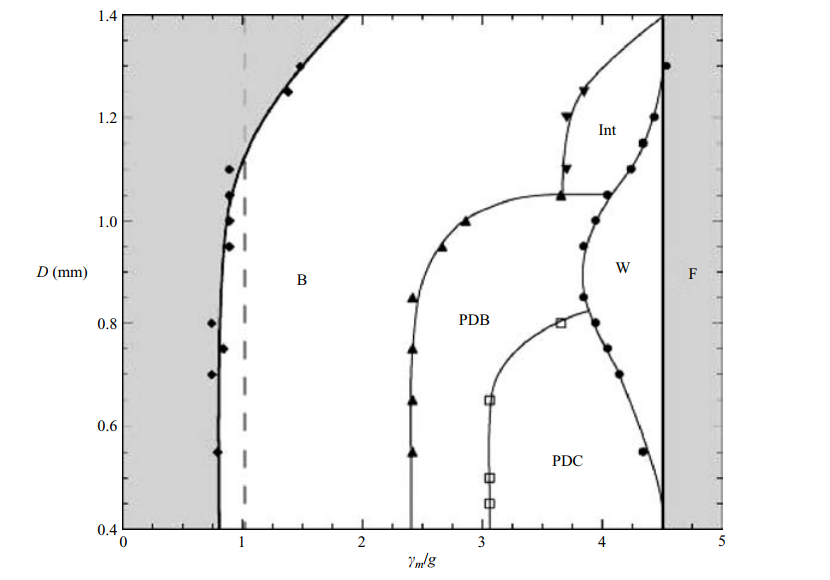
\includegraphics[width=12cm]{theory/regime}
\centering
\caption{A graph of droplet diameter against $\frac{\gamma_{m}}{g}$ for an oscillating droplet in a vibrating liquid. It illustrates the different vertical acceleration regimes: Bouncing (B), Walking (W), Faraday instability (F), Period Doubling (PDB), transition from Periodic to chaotic behaviour (PDC)  and Intermittent behaviour (Int).}
\centering
\label{regimes}
\end{figure}

Furthermore, droplets can also exhibit motion parallel to the droplet surface. Such droplets are labelled walkers, and like bouncing droplets, they exist in a certain $\frac{\gamma_{m}}{g}$ regime, just below the onset of the Faraday instability. The Faraday instability is defined as the point at which a surface becomes spontaneously wavy. Just before its onset, a bouncing droplet has a period of motion twice that of its driving oscillation. It thus generates a damped travelling Faraday wave at each bounce, where Faraday waves are standing waves generated by a vibrating liquid. The subsequent landing then occurs on the reverse slope of this previously generated Faraday wave. This landing generates another travelling Faraday wave, and causes the droplet to perform a parabolic bounce, causing motion parallel to the surface. An intuitive way to understand this motion is to imagine jumping on a trampoline. Each time you land on the trampoline, a wave is generated. If you land again anywhere but at the centre of this wave, you spring off again, and your motion has a slight horizontal component, allowing you to travel around the trampoline. As the wave you generate when landing travels, you constantly land on its side, therefore there is a constant horizontal motion, allowing you to 'walk' around the trampoline. This motion is illustrated in Figure \ref{walker}. 

\begin{figure}[ht]
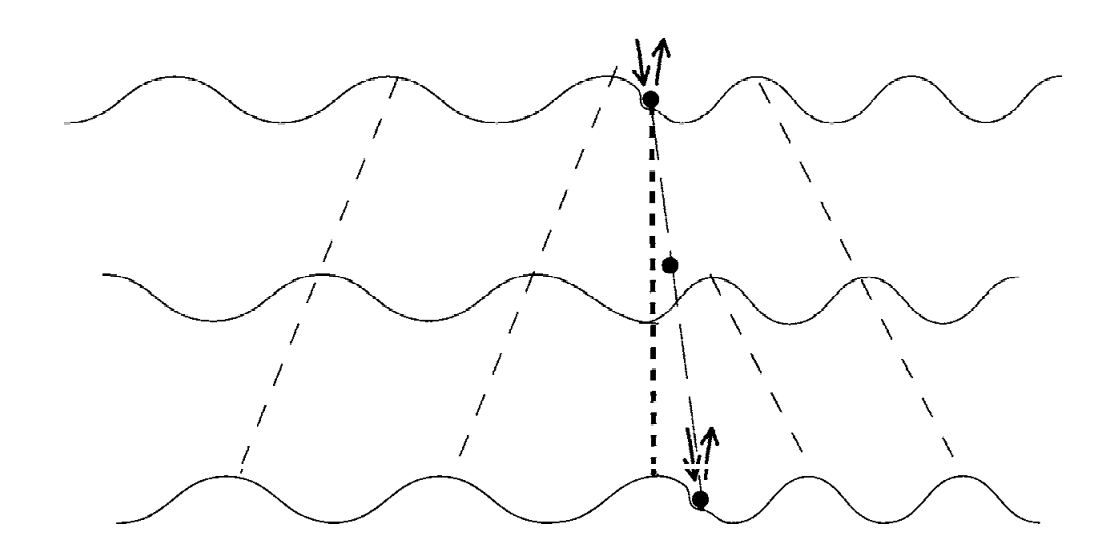
\includegraphics[width=12cm]{theory/walkingDroplet}
\centering
\caption{An illustration of a walking droplet's motion for subsequent bounces. The movement of droplet is exaggerated for visual purposes. In reality, wave amplitude decays with distance from droplet and is not necessarily constant; it is modulated by the driving force. }
\centering
\label{walker}

\end{figure}

Equations of motion for this droplet motion described above were taken from \cite{oza2013trajectory}, which showed that the surface wave produced on the $\textrm{n}^{\textrm{th}}$ impact of a particle at position $r_n$ and time $T_n$ on a surface oscillating vertically at $\omega$ above the Faraday threshold is given by (\ref{equ:heightSurfaceWave}). Here, $ h(\vec{r} , t)$ is the height of the wave at $\vec{r}$, $J_0$ is a Bessel function of the first kind, and wave number $k$ satisfies the relation $ J_0 \left( k \vec{r_0} \right) = 0$. $\vec{r_0}$ is a numerical cutoff parameter, while the amplitude of the wave, A is material specific and determined by the system parameters used. The exponential decay term at the end of the equation describes the wave decaying over time at a rate determined by the memory $Me$ and period of particle $T_f$.

\begin{equation}
h_n(\vec{r} , t) = A J_o\left(k\left|\vec{r} - \vec{r_n}\right| \right) e^{-\frac{\left(t-T_n\right)}{T_f Me}}
\label{equ:heightSurfaceWave}
\end{equation}

The overall surface wave can thus be described by the sum of all waves produced by every prior impact. Assuming the particle only interacts with the surface once every period (when the particle is at its lowest point), the overall wave equation $h (\vec{x} , t)$ is thus given by (\ref{equ:heightSumSurfaceWaves}).

\begin{equation}
h(\vec{r} , t) = \sum_{n=-\infty}^{\frac{t}{T_f}} A J_o\left(k\left|\vec{r} - \vec{r_n}\right| \right) e^{-\frac{\left(t-n T_f\right)}{T_f\times Me}}
\label{equ:heightSumSurfaceWaves}
\end{equation}

Furthermore, we know that the surface wave needs to consider relativistic effects. The coordinate transform on the wave formed by the $n^{\textrm{th}}$ impact of a particle at some velocity v is as follows:
\begin{equation}
h_n(\vec{r} , t) = A_0 cos\left(\omega_0 t - \frac{\gamma^2 \omega_0 v}{c^2}\right) J_0\left(k \left| \left(\vec{r} - \vec{r_n}\right)^{\prime \prime}  \right| \right)e^{-\frac{\left(t-n T_f\right)}{T_f\times Me}}
\end{equation}

Where:
\begin{equation}
\gamma = \frac{1}{\sqrt{1-\frac{v^2}{c^2}}}
\end{equation}
\begin{equation}
\left(\vec{r} - \vec{r_n}\right)^{\prime \prime} = \gamma^2(\vec{r_v}-\vec{v}t)+\gamma\vec{r_{\perp}}
\end{equation}

$\vec{r_v}$ and $\vec{r_{\perp}}$ are the components of $\left(\vec{r} - \vec{r_n}\right)$ in the direction of velocity and perpendicular to velocity respectively.

The memory parameter,  $Me$ , represents the decay time of a wave produced from a given impact in terms of the time between each impact. It is defined by the ratio between the non-dimensional damping time $\tau$, and the Faraday period of the system $T_f$.
A droplet entering a walking state is a direct result of this memory parameter and can seen by the comparison of the high and low memory regimes \cite{couder11}.
In the high memory regime, the waves decay slowly, and so waves created in the distant past can still strongly influence the particle trajectory. However, in the low memory regime, the waves decay rapidly, so only waves created in the recent past can significantly influence the particle's trajectory. 